\documentclass[11pt]{article}
\usepackage{fancyhdr}
\usepackage[letterpaper, margin=1in]{geometry}
%\usepackage{indentfirst}
\usepackage{graphicx}
\usepackage{amsmath}
\usepackage{amssymb}
\usepackage{siunitx}
\sisetup{detect-weight=true, detect-family=true} % makes siunitx follow font formatting like bold, italic, etc.
\usepackage{cancel}
\usepackage{isotope}
\usepackage{listings}
\usepackage[dvipsnames,table]{xcolor}
\usepackage{xspace}
\usepackage{booktabs} % makes tables pretty
\usepackage{longtable} % for long tables
\usepackage{multirow} % makes tables pretty
\usepackage{multicol} % makes tables pretty
\usepackage{setspace}
\usepackage{subcaption}

\newcommand{\creflastconjunction}{, and\nobreakspace} % adds oxford comma to cleveref
\usepackage[utf8]{inputenc}
\usepackage{textcomp}
\usepackage{titlesec}
\usepackage{svg}
\usepackage{pdflscape} % makes pages landscape
\usepackage{mathtools}
\usepackage{enumitem}
\usepackage[T1]{fontenc}
\usepackage{tikz}

\usepackage{hyperref}
\usepackage{cleveref}


\doublespacing

% bib if needed
\bibliographystyle{ieeetr}


% fancy header stuff
\usepackage{fancyhdr}
\pagestyle{fancy}

\setlength{\headheight}{28pt}
\lhead{ME 568 / OC 674\\Spring 2022}
\chead{Assignment 4\\}
\rhead{Austin Warren\\Due May 24, 2022}

\begin{document}
	
	\begin{enumerate}
		% Part 1
		\item \textbf{Part 1:} Choose a time when the flow is strongly turbulent and evaluate the following:
		\begin{enumerate}
			\item First perform a Reynolds decomposition by defining the mean and perturbation $u$, $v$, $w$. Because the background state varies in $z$. Discuss any challenges you might have in doing decomposition.\par
			
			I chose the eighth time step ($t=\SI{3043.9}{\second}$) because it is far enough along to have turbulence. I also did my analysis only in the second $y$ plane. For the Reynolds decomposition, I decided to average over $x$, such that the mean velocity is only a function of $z$. I did this for the velocity in all three directions. The fluctuating values are then just the difference between the instantaneous velocity and the mean velocity. Normally, the Reynolds decomposition involves a time average, however in this case, the time steps are very far apart and do not provide a sufficient number of data points to provide a good average. The mean as a function of $z$ and $t$ works well because the flow in the $x$-direction is relatively constant at each $z$ value, especially in the early stages of the simulation. \Cref{fig:Vel 3043,,fig:Vel avg 3043,,fig:Vel prime 3043} show the instantaneous, mean, and fluctuating velocities, respectively. The mean velocity is plotted as a function of $z$ only, while the instantaneous and fluctuating velocities are plotted as functions of both $x$ and $z$. (Please note that I will still play with the limits of the plots to make them look the best, but I wanted to have something today to get feedback on.)
			
			
			\begin{figure}[htbp]
				\centering
				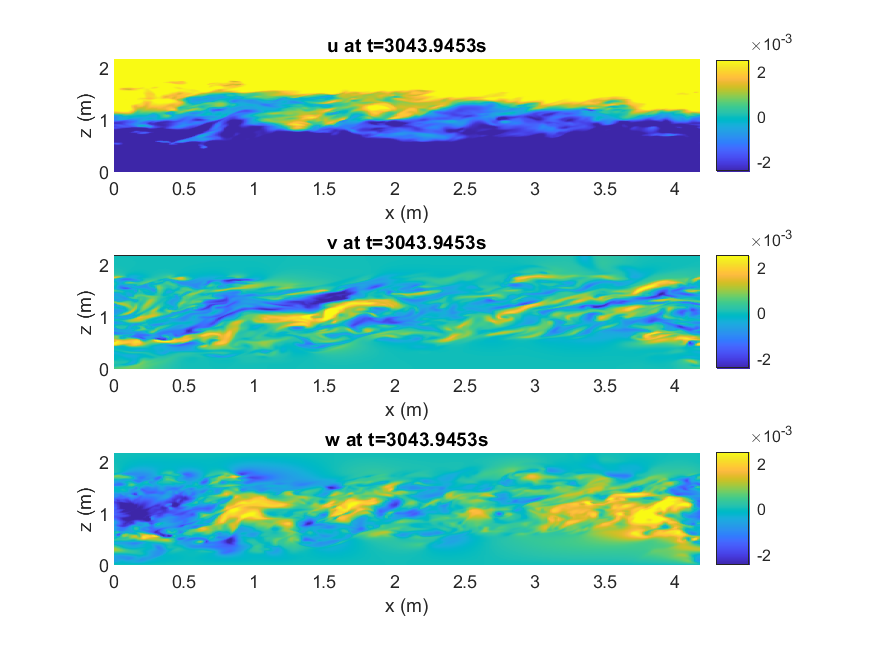
\includegraphics[width=\textwidth]{1-plots/Vel_plot_3043.png}
				\caption{Instantaneous velocity at $t=\SI{3043.9}{\second}$.}
				\label{fig:Vel 3043}
			\end{figure}
		
			\begin{figure}[htbp]
				\centering
				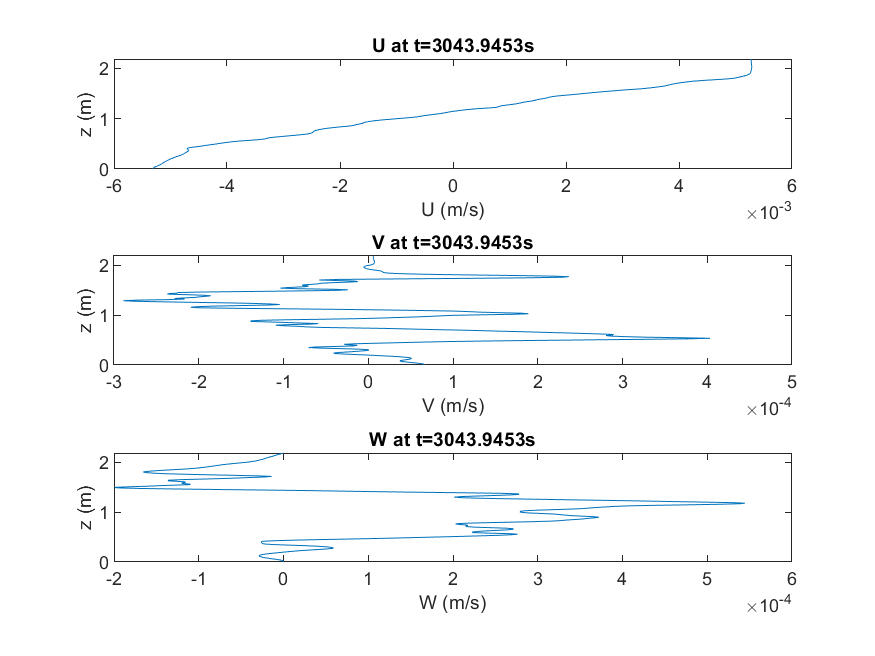
\includegraphics[width=\textwidth]{1-plots/Vel_avg_plot_3043.png}
				\caption{Mean velocity at $t=\SI{3043.9}{\second}$.}
				\label{fig:Vel avg 3043}
			\end{figure}
		
			\begin{figure}[htbp]
				\centering
				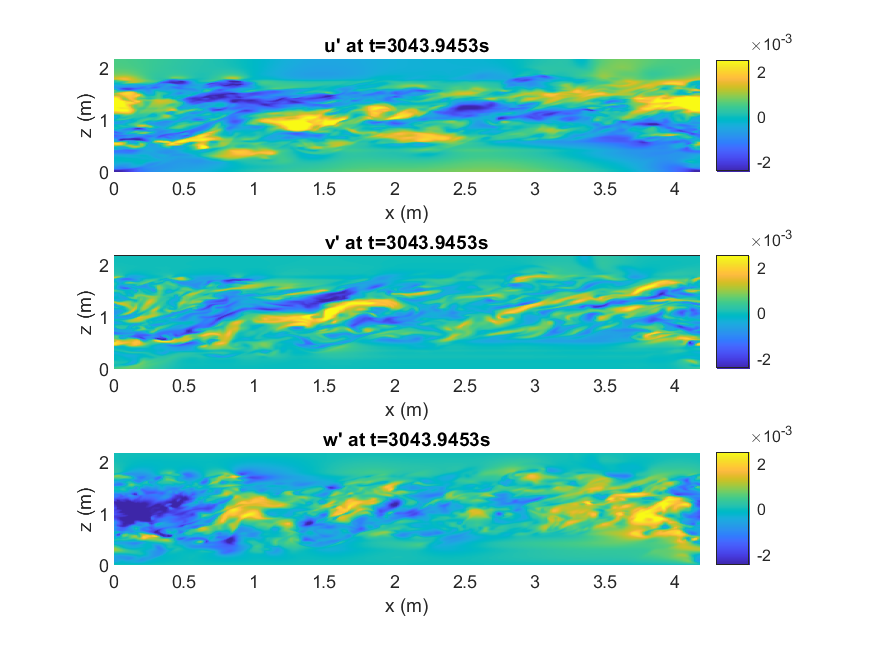
\includegraphics[width=\textwidth]{1-plots/Vel_primes_plot_3043.png}
				\caption{Fluctuating velocity at $t=\SI{3043.9}{\second}$.}
				\label{fig:Vel prime 3043}
			\end{figure}
			
			
			\clearpage
			\item Now that you have decomposed the velocity, compute the individual components of the turbulent kinetic energy and the Reynolds stresses. Discuss any significant features of the patterns or magnitudes.\par
			
			To calculate the TKE and the Reynolds stresses, I multiplied the fluctuating velocities together at each point in the time step. For the TKE, shown in \Cref{fig:tke 3043}, I plotted the individual components, as well as the total TKE as functions of $x$ and $z$. I still need to fix the limits for the plots so each plot uses the same colors for their values, but I did not know before plotting what the values would be. From the magnitudes I can see currently, the $x$-direction TKE is the largest and contributes the most to the total. The other two components have contributions that can be seen on the total TKE plot, but the overall shape matches with the $x$-component. \Cref{fig:reynolds 3043} shows the components of the Reynolds stress, without being multiplied by density. Again, I need to do more work on the axis limits on these plots, but it looks like the $u^{\prime}$ components are the strongest, with being much larger than the others. I would expect that the $u^{\prime}w^{\prime}$ component is the largest since the $x$-direction is the direction of the main flow and the $z$-direction is the direction where the turbulence starts. (I need to make this plot look better, it is difficult to make out any important detail.)
			
			\begin{figure}[htpb]
				\centering
				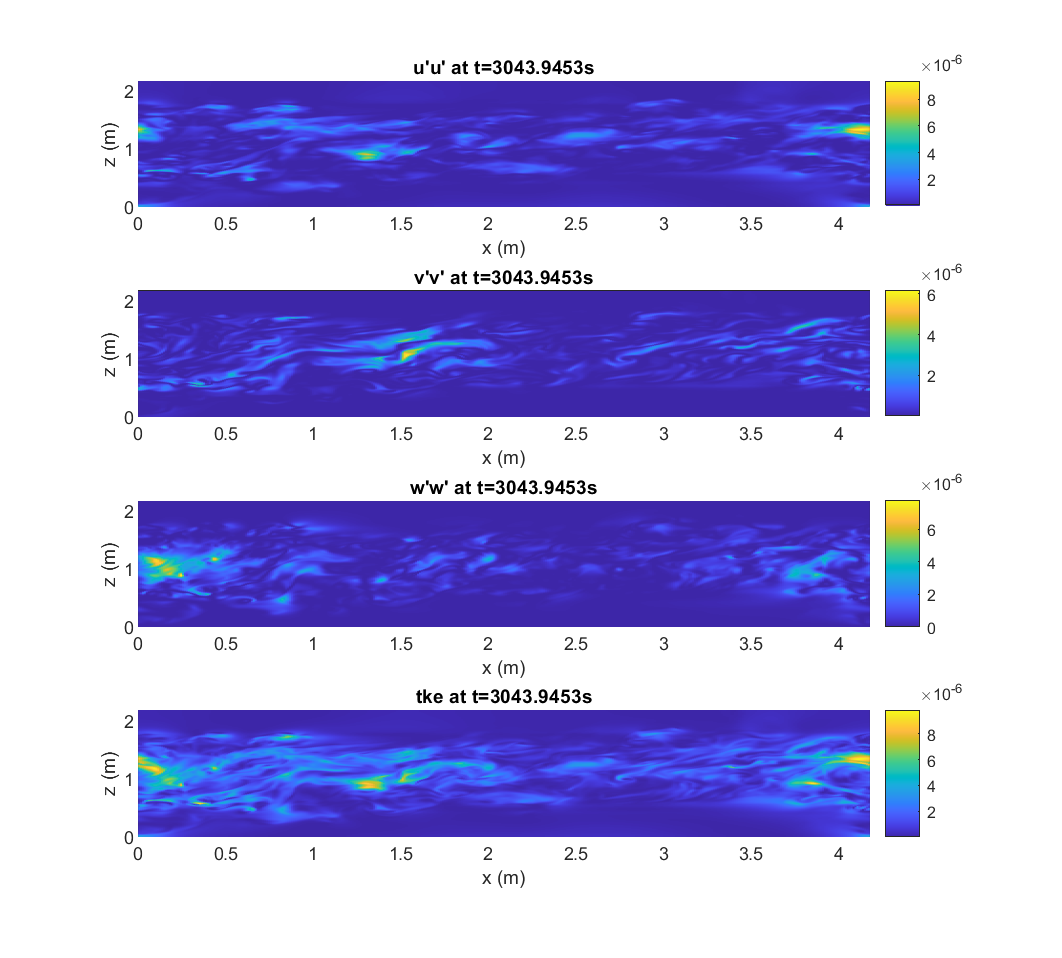
\includegraphics[width=\textwidth]{1-plots/tke_plot_3043.png}
				\caption{TKE at $t=\SI{3043.9}{\second}$.}
				\label{fig:tke 3043}
			\end{figure}
		
			\begin{figure}[htbp]
				\centering
				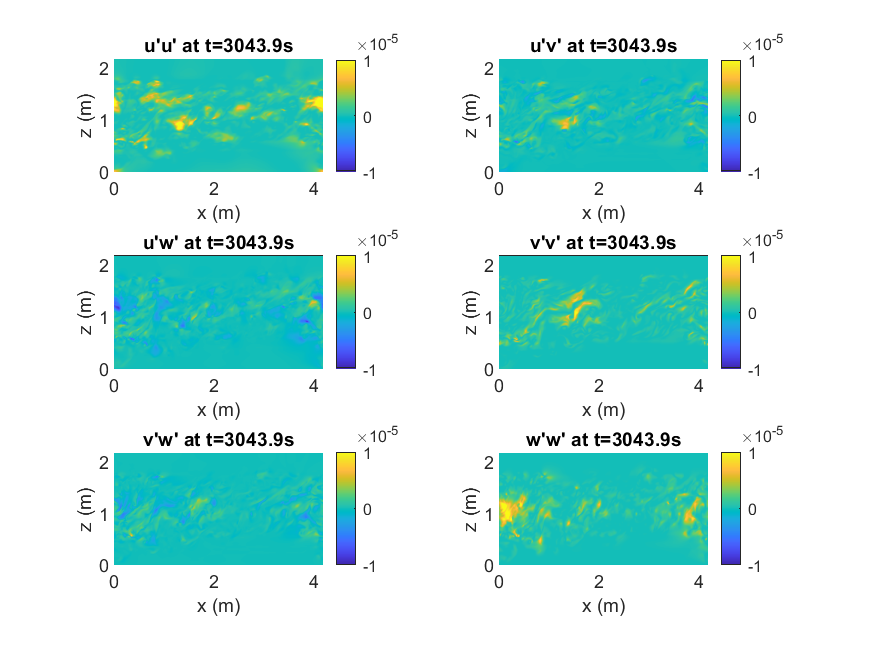
\includegraphics[width=\textwidth]{1-plots/ReynoldsStress_plot_3043.png}
				\caption{Reynolds stresses at $t=\SI{3043.9}{\second}$.}
				\label{fig:reynolds 3043}
			\end{figure}
			
			\clearpage
			\item Perform the same set of calculations for an earlier time in the flow (when the turbulence is perhaps less homogeneous). Discuss any differences in the character of the flow and/or the components of the tke and Reynolds stresses.\par
			
			I have not done this for a second time step yet, but the process would be the same. I would expect that the components of fluctuating velocity, stress, and TKE in the $z$ and $y$ directions to be less than they are at the later time step, since they are increased by the turbulence.
			
			
			
		\end{enumerate}
	
		\clearpage
		% Part 2
		\item \textbf{Part 2:} For now neglect the buoyancy contributions and
		\begin{enumerate}
			\item compute the shear production and dissipation throughout the domain at some point in time. Determine a horizontal and volume average of each. Does production balance dissipation?\par
			
			This is the part that I am most unsure about currently. I am not sure that I am calculating $S_{ij}$ and $s_{ij}$ correctly. Beginning with the definitions of shear production and dissipation from the TKE equation, we have:
			\begin{equation}
				P = - \overline{u_i u_j} S_{ij}\:,
				\label{eq:production}
			\end{equation}
			and
			\begin{equation}
				\epsilon = 2\nu \overline{s_{ij} s_{ij}}\:.
				\label{eq:dissipation}
			\end{equation}
			The definition for $S_{ij}$:
			\begin{equation}
				S_{ij} = \frac{1}{2} \left( \frac{\partial U_i}{\partial x_j} + \frac{\partial U_j}{\partial x_i} \right)\:.
				\label{eq:Sij def}
			\end{equation}
			I initially thought that because I am ignoring the $y$-direction, the only component I was interested in was the $S_{13}$ term, which gives the following for the mean.
			\begin{equation}
				S_{13} = \frac{1}{2} \left( \frac{\partial U_1}{\partial x_3} + \frac{\partial U_3}{\partial x_1} \right)
			\end{equation}
			Because I averaged over $x$, there cannot be a partial derivative in the $x$-direction, so this reduces to:
			\begin{equation}
				S_{13} = \frac{1}{2} \frac{\partial U}{\partial z}\:.
			\end{equation}
			The fluctuating term would keep this $x$ derivative because it is not averaged.
			\begin{equation}
				s_{13} = \frac{1}{2} \left( \frac{\partial u^{\prime}}{\partial z} + \frac{\partial w^{\prime}}{\partial x} \right)
			\end{equation}
			I calculated the production and dissipation using these definitions, but after discussing with other students, I was convinced that $S_{ij}$ has more terms, so I calculated the production and dissipation using the following definitions. The additional terms come from the fact that the strain is a second order tensor and therefore has nine terms, but $S_{ij}$ is just the symmetrical part, so its actually three unique terms, which then reduce down due to neglecting the $y$-direction and averaging over $x$.
			\begin{equation}
				S_{ij} =  \frac{1}{2} \left( \frac{\partial U_1}{\partial x_2} + \frac{\partial U_2}{\partial x_1} \right) + \frac{1}{2} \left( \frac{\partial U_2}{\partial x_3} + \frac{\partial U_3}{\partial x_2} \right) + \frac{1}{2} \left( \frac{\partial U_3}{\partial x_1} + \frac{\partial U_1}{\partial x_3} \right)
			\end{equation}
			\begin{equation}
				S_{ij} = \frac{1}{2} \left( \frac{\partial U}{\partial z} + \frac{\partial V}{\partial z} \right)
			\end{equation}
			Now the fluctuating part.
			\begin{equation}
				s_{ij} = \frac{1}{2} \left( \frac{\partial u^{\prime}}{\partial z} + \frac{\partial w^{\prime}}{\partial x} + \frac{\partial v^{\prime}}{\partial z} + \frac{\partial v^{\prime}}{\partial z} \right)
			\end{equation}
			I do not think these new definitions are correct. I am not very familiar with tensor math, but just adding the terms together doesn't seem right. Only using the 1-3 component makes sense to me, since that is what we are looking at mostly, but I am not sure. I have probably thought about it too much. (Hopefully you can provide some insight into which of these paths is correct, or at least in the right direction.) I did not compare my plots with both methods yet, so I do not know how much impact it has. Other students I have worked with did compare these two methods and the results seem very close, with some minor differences that are expected by added more terms. \Cref{fig:prod diss 3043} shows the production and dissipation as functions of $x$ and $z$. As with all of the other plots, I need to adjust the axes so they are the same scale for easier comparison, but it does appear that the shape of the production follows the dissipation (or the other way around, they look similar in shape). I would guess that they do not exactly balance each other, but are probably close, just from looking at the plots. To average the production and dissipation, I averaged over $x$ for each $z$ for the horizontal average (the same type of average as I performed for the velocity); for the volume average, I averaged the horizontal average values together to get one number. The total volume average values can be seen in \Cref{tab:prod diss}. They are the same order of magnitude, but the production is almost twice as large as the dissipation.
			
			
			\begin{figure}[htbp]
				\centering
				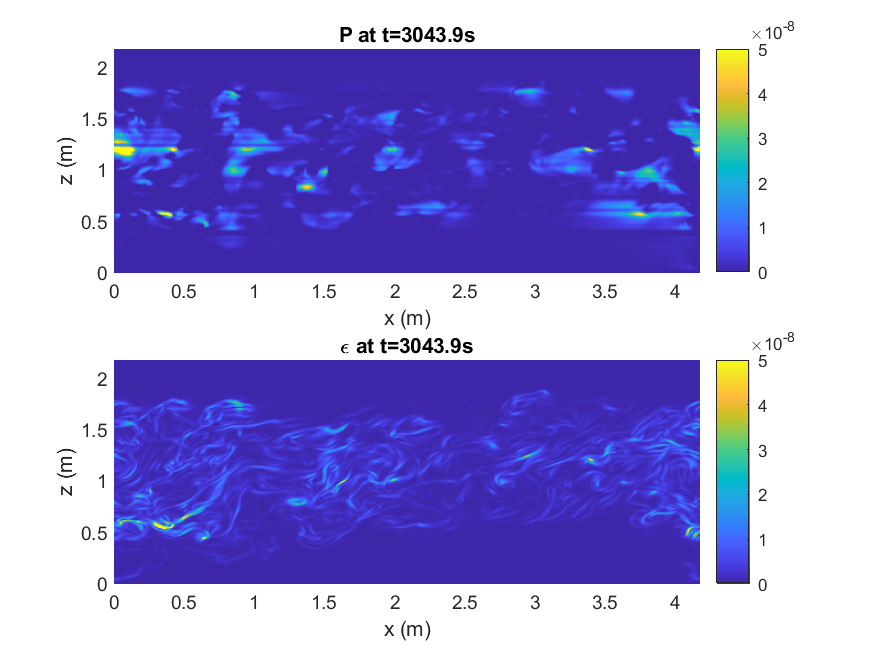
\includegraphics[width=\textwidth]{1-plots/prod_diss_plot_3043.png}
				\caption{Production and dissipation at $t=\SI{3043.9}{\second}$.}
				\label{fig:prod diss 3043}
			\end{figure}
		
			\begin{table}[htbp]
				\centering
				\caption{Volume averaged production and dissipation at $t=\SI{3043.9}{\second}$.}
				\begin{tabular}{cc}
					\toprule
					Parameter & Value\\
					\midrule
					P & 2.6973e-10\\
					$\epsilon$ & 1.5112e-10\\
					\bottomrule
				\end{tabular}
				\label{tab:prod diss}
			\end{table}
			
			
			\clearpage
			\item Once you are satisfied that you can compute production and dissipation (i.e., (a) above), compute the average of each for every timestep and plot a time series. Does production equal dissipation on average? Write a paragraph describing the production and dissipation evolution.
		\end{enumerate}
	
	
		\clearpage
		% Part 3
		\item \textbf{Part 3:} Now consider the buoyancy production term.
		\begin{enumerate}
			\item Compute time-integrals of the spatially-integrated buoyancy production $J_b$ and compare this to shear production and dissipation. Does this help to account for any mismatches above? If there are mismatches and you can't close the energy budget, explain what might be the problem.
			
			
			\item  Now try to compare these to the integrated TKE production and the total change in potential energy due to mixing within the simulation domain. Can you close an energy budget, and if not, what might be the problem? What is the mixing efficiency? Which measure of the total mixing is most robust?
		
		\end{enumerate}
		
	\end{enumerate}
		
	
	
	
	
	
	
	
	
	
\end{document}